\documentclass{beamer}

\mode<presentation> {

    \usetheme{Madrid}
    \usecolortheme{beaver}
}

\usepackage{graphicx}

%--------------------------------------------------
% Title Page
%--------------------------------------------------

\title[git]{A short introduction to git}
\author{John Ladan}
\institute[Waterloo]{University of Waterloo\\john@ladan.ca}
\date{\today}

\begin{document}

\begin{frame}
    \titlepage
\end{frame}

\begin{frame}
    \frametitle{Overview}
    \tableofcontents
\end{frame}

%--------------------------------------------------
% Presentation slides
%--------------------------------------------------

\section{What is git?}

\begin{frame}
    \frametitle{According to git-scm.com}
    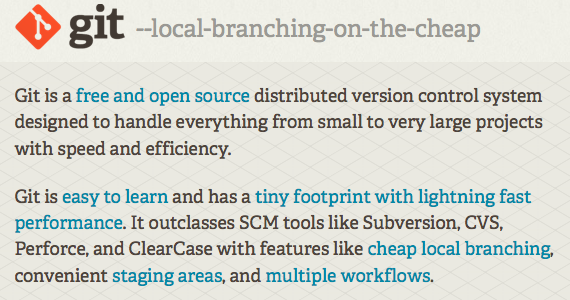
\includegraphics{figures/git-homepage}
\end{frame}

\begin{frame}
    \frametitle{According to wikipedia.org}
    Git (/ɡɪt/) is a distributed revision control system with an emphasis on speed, data integrity, and support for distributed, non-linear workflows. Git was initially designed and developed by Linus Torvalds for Linux kernel development in 2005, and has since become the most widely adopted version control system for software development.

    As with most other distributed revision control systems, and unlike most client–server systems, every Git working directory is a full-fledged repository with complete history and full version-tracking capabilities, independent of network access or a central server. Like the Linux kernel, Git is free software distributed under the terms of the GNU General Public License version 2.
\end{frame}

\begin{frame}
    \frametitle{Features}
    \begin{itemize}
        \item Fast
        \item Nonlinear development (via rapid branching, and DAG based structure)
        \item Distributed -- each copy of the repo is complete by itself
            \begin{itemize}
                \item each copy of the repo is itself a repo
                \item changes can be pushed/pulled to any other instance
                \item do not need network access
            \end{itemize}
        \item Ubiquitous
    \end{itemize}
\end{frame}

% Probably something about github here



\section{Cloning a Repo}

\section{Making Changes}

\section{Starting Your Own}

\section{Version Control}

\section{In Practice}
